% !TEX root = ../bachlor-arbeit.tex
Having done the necessary preliminary considerations we can now start implementing the algorithm. It is organized into separate software modules defined by their inputs and outputs. The composition of these modules to the complete algorithm is shown in figure \ref{fig:al:algo} and the individual modules will be discussed in the following sections. Each section will start with the input and output to that module. The sections are ordered as their corresponding modules appear in the algorithm, with the exception of the SASA module, which was already discussed in the background section \ref{sec:SASA}.

\begin{figure}[H]
    \centering
    \includegraphics[width=.9\linewidth]{al_algo_new}
    \caption[]{The algorithm tries to find to a given transmission spectrum $I$ the design parameters $\mc D$ of a two layer meta surface stack which can reproduce this target. The input spectrum is passed to a convolutional neural network which outputs its guess for the stack and layer parameters. The Database module looks at the two sets of layer parameters and interpolates between stored $S$-matrices to give an estimate for the two $S$-matrices describing the layers. The SASA module calculates the resulting current transmission spectrum and passes it to the optimizer. This last module compares it to the target spectrum and adjusts the continuous parameters to minimize the difference between the two spectra.}
    \label{fig:al:algo}
\end{figure}
\vspace{0.35cm}


\begin{tabular}{ll}
    \vspace{0.35cm}
    \hyperref[sec:NN]{NN}: &
    \begin{tabular}[t]{@{}l@{}}
        convolutional neural network trained to map spectra to stack and \\ layer parameters
    \end{tabular}\\
    %
    \vspace{0.35cm}
    \hyperref[sec:DB]{DB}: &
    database of pre-simulated single layers\\
    %
    \vspace{0.35cm}
    \hyperref[sec:SASA]{SASA}: &
    module calculating $\hat{S}_\s{stack} = \hat{S}_\s{stack}(\hat{S}_1, \, \hat{S}_2, \, \varphi, \, h)$\\
    %
    \vspace{0.35cm}
    \hyperref[sec:opt]{Opt}: &
    \begin{tabular}[t]{@{}l@{}}
        optimizer changing the continuous parameters to minimize the difference \\
        between the current and target spectrum
    \end{tabular}\\
    %
    \vspace{0.35cm}
    $\hat{S}_1, \, \hat{S}_2$ &
    S-matrices of the top and bottom layer\\
    %
    \vspace{0.35cm}
    $\mc L_1 , \, \mc L_2$ &
    \begin{tabular}[t]{@{}l@{}}
        two sets of layer parameters where
        $\mc L = (w, \, l, \, t, \, \Lambda, \, m, \, g)$ \\
        $w$...width, $l$...length, $t$...thickness, $\Lambda$...Period,
        $m$...material, $g$...geometry
    \end{tabular}\\
    %
    \vspace{0.35cm}
    $\mc S$ &
    \begin{tabular}[t]{@{}l@{}}
        stack parameters $\mc S = (d, \varphi)$ where \\
        $d$...distance between layers, $\varphi$...rotation angle\\
    \end{tabular}\\
    %
    \vspace{0.35cm}
    optimization loop & this loop is repeated until the target accuracy is reached\\
    %
    \vspace{0.35cm}
    $I$ & input transmission spectrum\\
    %
    \vspace{0.35cm}
    $\mc D$ & output design parameters\\
\end{tabular}
